\subsubsection{a)}
The heat equation 

\begin{equation}
    u_t = u_{xx}, \hspace{1mm} u_x(0,t) = u_x(1,t) = 0, \hspace{1mm} u(x,0) = 2\pi x - \sin{(2\pi x)},
\label{heat_eq}
\end{equation}
on $x \in [0,1], t > 0$, with Neumann boundary conditions will be studied in this problem. An equidistant grid of points in the $x$-direction

\begin{equation*}
    x_0 = 0, \, x_1 = \frac{1}{M+1}, \, \dots, \, x_M = \frac{M}{M+1}, \, x_{M+1} = 1,
\end{equation*}
will be utilized when computing the numerical solution. Semi-discretization will be used to solve the problem numerically; the PDE is discretized in the $x$-direction, before the resulting ODEs are solved with first and second order methods in time. Let $v_m(t) \approx u(x_m,t)$ for $0 \le m \le M + 1$, i.e. the numerical solution along the line $(x_m, t)$ is denoted by $v_m(t)$. For ease of notation, the explicit $t$-dependency may not be included in the following, i.e let $v_m := v_m(t)$. Furthermore, we require that 

\begin{equation}
    \dot{v}_m = \frac{1}{h^2} \delta^2 v_m = \frac{1}{h^2}(v_{m-1} - 2v_m + v_{m+1}) \quad 1 \le m \le M,
\label{cd}
\end{equation}
where $\dot{v}_m = \frac{\mathrm{d}v_m(t)}{\mathrm{d}t}$ and $h = \frac{1}{M+1}$. The boundary conditions will be discretized with both first and second order methods.
\subsubsection{First Order Discretization of Boundary Conditions}


%Discretization in the x-direction, using a forward difference scheme, gives a method of order one in x. The forward difference operator will be denoted by $\Delta u(x) = u(x+h) - u(x)$. It can be shown by Taylor expansion that $\frac{\Delta^2u(x)}{h^2}$ is an approximation of order 1 to the second derivative $u_{xx}$. This gives


%\begin{equation}
    %u_t(x_m, t) = u_{xx}(x_m, t) = \frac{1}{h^2}\Delta^2u(x_m,t) + %h\partial_x^3u(x_m,t) + \dots.
%\end{equation}

%In a similar fashion, the boundary conditions can be discretized to the first order by

%\begin{equation}
%\begin{split}
    %\partial_xu(0,t) &= 0, \\
    %\Delta u(x_0, t) &= 0 + \frac12h\partial_x^2u(x) + \dots, \\
    %\frac{u_1-u_0}{h} &= \frac12h\partial_x^2u(x) + \dots, 
%\end{split}
%\end{equation}

%and 

%\begin{equation}
%\begin{split}
    %\partial_xu(1,t) &= 0, \\
    %\Delta u(x_{M+1}, t) &= 0 + \frac12h\partial_x^2u(x) + \dots, \\
    %\frac{u_{M+2}-u_{M+1}}{h} &= \frac12h\partial_x^2u(x) + \dots, 
%\end{split}
%\end{equation}

%where we have added a fictitious node at $x_{M+2} = 1 + h$. \textcolor{red}{Usikker på om vi kunne brukt en backwards difference her i stedet, men prøver dette først i så fall. I ettertid ser det ut som at dette gjøres på side 44 i heftet, well well. Kunne jo også brukt noe annet en forward difference også, for å få en metode av orden 1.} 

%Let $v_m(t) \approx u(x_m,t)$ for $0 \le m \le M + 1$. For the method to be of order 1 and to avoid fictitious nodes, we use forward differences is the $M$ first points and backward differences in the two last points. The discretization becomes

%\begin{equation}
%\begin{split}
%\label{firstOrder}
     %&\dot{v}_m = \frac{1}{h^2}\Delta^2v(x_m,t), \quad 0\leq m \leq M-1, \\
     %&\dot{v}_m = \frac{1}{h^2}\nabla^2v(x_m,t), \quad m = M, M + 1, 
%\end{split}
%\end{equation} 


First, the left and right end points are discretized with forward and backward differences, respectively. Using the above notation, require that 

\begin{equation}
\begin{split}
     &\dot{v}_m = \frac{1}{h^2} \delta^2 v_m \quad 1 \le m \le M, \\
     &\dot{v}_0 = \frac{1}{h^2}\Delta^2v_0 \\
     &\dot{v}_{M+1} = \frac{1}{h^2}\nabla^2v_{M+1}, 
\label{diff1}
\end{split}
\end{equation} 
The boundary conditions are also discretized with forward and backward differences, which yields the following first order approximations in $h$

\begin{equation}
\begin{split}
     &-\frac{v_1-v_0}{h} = 0, \\ 
     &\frac{v_{M+1}-v_{M}}{h} = 0.
\label{bc1}
\end{split}
\end{equation} 
Combining (\ref{diff1}) and (\ref{bc1}) gives

\begin{equation}
\begin{split}
     &\dot{v}_0 = \frac{1}{h^2}(v_2 - v_0), \\
     &\dot{v}_{M+1} = \frac{1}{h^2}(v_{M-1}-v_{M+1}).
\label{bc2}
\end{split}
\end{equation} 
Finally, a linear system of ordinary differential equations can be assembled as 

\begin{equation*}
    \dot{\boldsymbol{v}} = \frac{1}{h^2}Q\boldsymbol{v},
\end{equation*}
where 

\begin{equation*}
Q = \begin{pmatrix}
    -1 & 0 & 1 & & \\
     & 1 & -2 & 1 & \\
    & & \ddots & \ddots & \ddots &\\
     & & & 1 & -2 & 1 \\
     &  & & 1& 0 & -1
    \end{pmatrix} \in \mathbb{R}^{(M+2) \times (M+2)}, \, 
    \dot{\boldsymbol{v}} = \begin{pmatrix}
    \dot{v_0} \\
    \dot{v_1} \\
    \vdots \\
    \dot{v}_{M+1} 
    \end{pmatrix} \in \mathbb{R}^{M+2}.
\end{equation*}

\subsubsection{Second Order Discretization of Boundary Conditions}

The same notation as above is adopted in this section. In order to use central differences on the boundary conditions, the fictitious nodes $x_{-1} = -h$ and $x_{M + 2} = 1 + h$ are introduced. The discretization of the boundary conditions becomes

\begin{equation}
    -\frac{v_1 -v_{-1}}{2h} = \frac{v_{M+2} - v_M}{2h} = 0.
\label{bc}
\end{equation}
Also, let

\begin{equation}
    \dot{v}_m = \frac{1}{h^2}(v_{m-1} - 2v_m + v_{m+1}) \quad 0 \le m \le M + 1.
\label{cd}
\end{equation}
Combining (\ref{bc}) with (\ref{cd}) gives $\dot{v}_0 = \frac{2}{h^2}(v_{1} - v_{0})$ and $\dot{v}_{M+1} = \frac{2}{h^2}(v_{M} - v_{M+1})$. Thus, the following system of equations

\begin{equation*}
    \dot{\boldsymbol{v}} = \frac{1}{h^2}Q\boldsymbol{v},
\end{equation*}
where 
\begin{equation*}
Q = \begin{pmatrix}
    -2 & 2 & & & \\
    1 & -2 & 1 & & \\
    & \ddots & \ddots & \ddots &\\
     & & 1 & -2 & 1 \\
     &  & & 2 & -2
    \end{pmatrix}, 
\end{equation*}
is constructed.

\subsubsection{Solution of the System of ODEs}
After a discretization of the boundary conditions is chosen and the system of ODEs

\begin{equation*}
    \dot{\boldsymbol{v}} = \frac{1}{h^2}Q\boldsymbol{v},
\end{equation*}
is assembled, a procedure for calculating the evolution of $\boldsymbol{v}$ in time needs to be chosen. This can be done with the trapezoidal rule, which amounts to the Crank-Nicolson method (hereafter denoted by CN). The Backward Euler method (hereafter denoted by BE) can also be used. Letting  $\boldsymbol{V}^0 = (u(x_0,0), \dots, u(x_{M+1},0))^T$, CN may be written as

\begin{equation*}
    \boldsymbol{V}^{n+1} = \boldsymbol{V}^n + \frac{k}{2}\left(\frac{1}{h^2}Q\boldsymbol{V}^n + \frac{1}{h^2}Q\boldsymbol{V}^{n+1} \right), 
\end{equation*}

\noindent where $k=\frac{T}{N}$ is the step length in time and $n$ denotes the current iteration. The system of equations is solved iteratively from $n=0$ to $n=N-1$ until the solution at $t_N=T$ is found. Equivalently, the method can be written as

\begin{equation}
    (I - \frac{k}{h^2}Q)\boldsymbol{V}^{n+1} = (I + \frac{k}{h^2}Q)\boldsymbol{V}^n \quad (\text{Crank-Nicolson}).
    \label{CN}
\end{equation}
Moreover, BE can be written as

\begin{equation}
    (I - \frac{k}{h^2}Q)\boldsymbol{V}^{n+1} = \boldsymbol{V}^n \quad (\text{Backward Euler}).
    \label{BE}
\end{equation}

 \noindent The local truncation error of CN and BE with second order discretization of boundary conditions are

\begin{equation}
    \begin{split}
        \tau_{CN} &= \mathcal{O}(k^2 + h^2), \\
        \tau_{BE} &= \mathcal{O}(k + h^2),
    \end{split}
\label{orders}
\end{equation}
respectively. These truncation errors can be shown using Taylor expansions around $(x_m, t_n)$. Inserting the exact solutions $\boldsymbol{U}^n = (u(x_0,t_n), \dots, u(x_{M+1},t_n))^T$ into BE gives the truncation error

\begin{equation*}
    k\tau_{BE} = (I - \frac{k}{h^2}Q)\boldsymbol{U}^{n+1} - \boldsymbol{U}^n.
\end{equation*}

\noindent Considering the system before boundary conditions are implemented, it can be written row-wise as 

\begin{equation*}
\begin{split}
    k\tau_{BE} &= (1 - \frac{k}{h^2}\delta_x^2)u_m^{n+1} - u_m^n, \quad 0 \leq m \leq M + 1\\
    &= \left(1 - k(\partial_x^2 + \mathcal{O}(h^2))(1 + k\partial_t + \frac{1}{2}k^2\partial_t^2 + \mathcal{O}(k^3))\right)u_m^n - u_m^n \\
    &= \left(k\partial_t + \frac{1}{2}k^2\partial_t^2 - k(\partial_x^2 + \mathcal{O}(h^2)) - k^2(\partial_x^2 + \mathcal{O}(h^2))\partial_t + \mathcal{O}(k^3)\right)u_m^n \\
    &= \left(-\frac{1}{2}k^2\partial_t^2 + \mathcal{O}(kh^2)\right)u_m^n \\
    &= \mathcal{O}(k^2 + kh^2), 
\end{split}
\end{equation*}
which shows that $\tau_{BE} = \mathcal{O}(k + h^2)$. A similar proof can be applied to show the order of the local truncation of CN \cite{Owren}. 

The numerical solution using CN (with second order discretization of boundary conditions) is plotted in figure \ref{2a_sol}.

\begin{figure}
\centering
\subfloat[Numerical Solution]{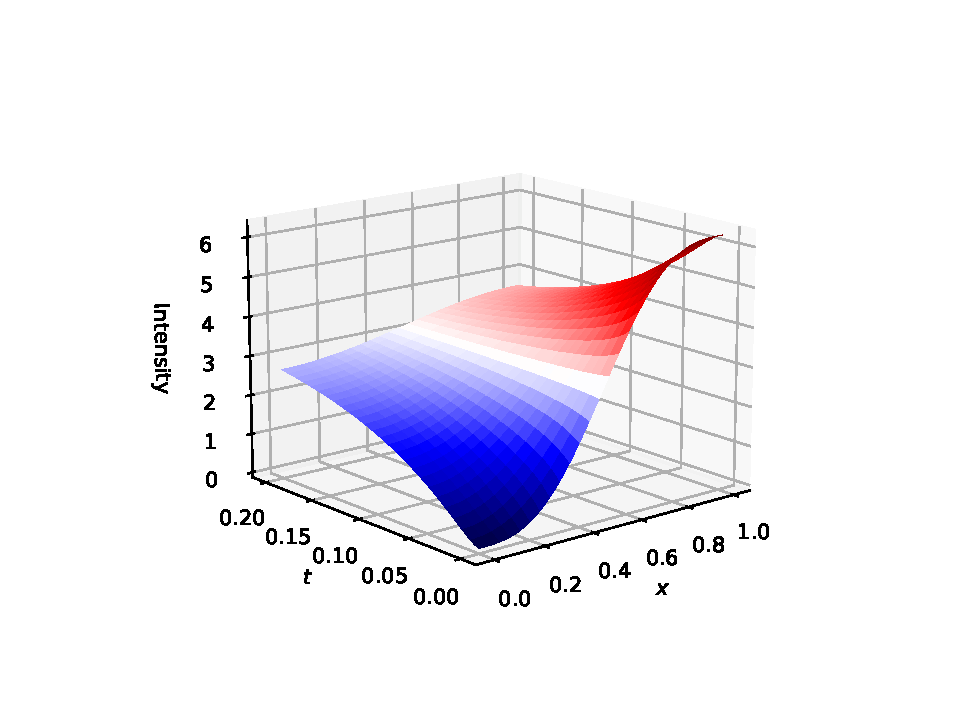
\includegraphics[width=0.9\linewidth]{plots/2a_sol.pdf}\label{2a_sol}}\hspace{0mm}
\subfloat[Relative error with $h$-refinement, 1st and 2nd order discretization of BC's]{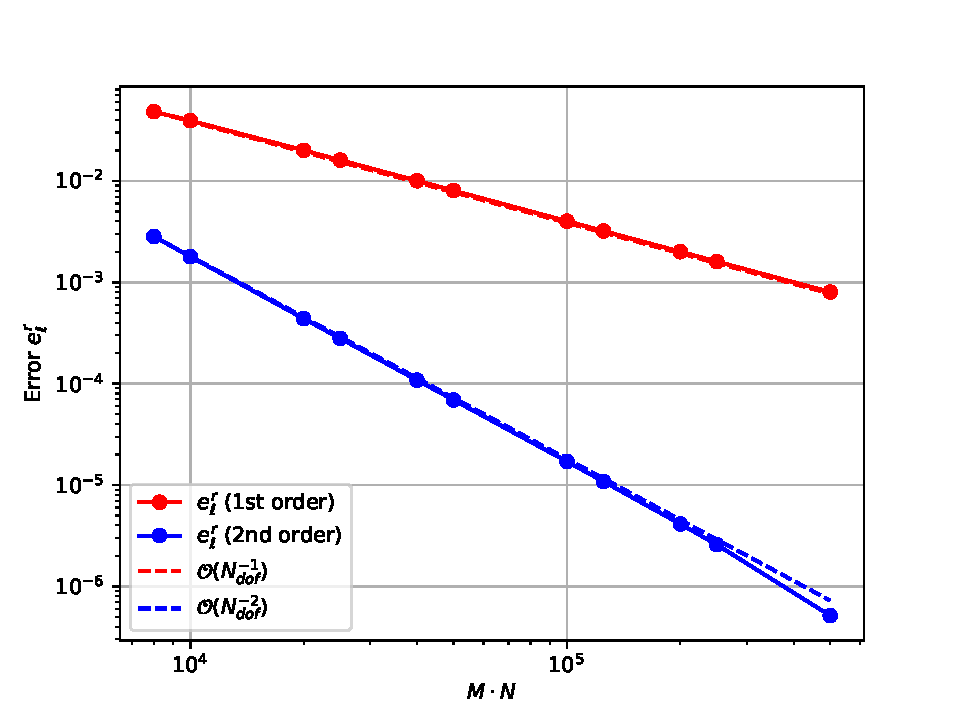
\includegraphics[width=0.85\linewidth]{plots/2a_comp.pdf}\label{2a_comp}}\hspace{0mm}
\caption{Heat equation with two Neumann boundary conditions and initial condition $u(x,0) = 2\pi x - \sin{(2\pi x)}$ on $x \in [0,1]$ and $t \in [0,0.2]$. The numerical solution, calculated using CN with $M=N=50$ and a second order discretization of the boundary conditions, is plotted in (a). The relative error with $h$-refinement for first and second order discretizations of the boundary conditions, is plotted in (b). CN was used also here with $N=1000$. The $x$-axis shows the number of degrees of freedom in the linear system.}
\end{figure}

\begin{comment}
\begin{figure}[t]
    \centering
    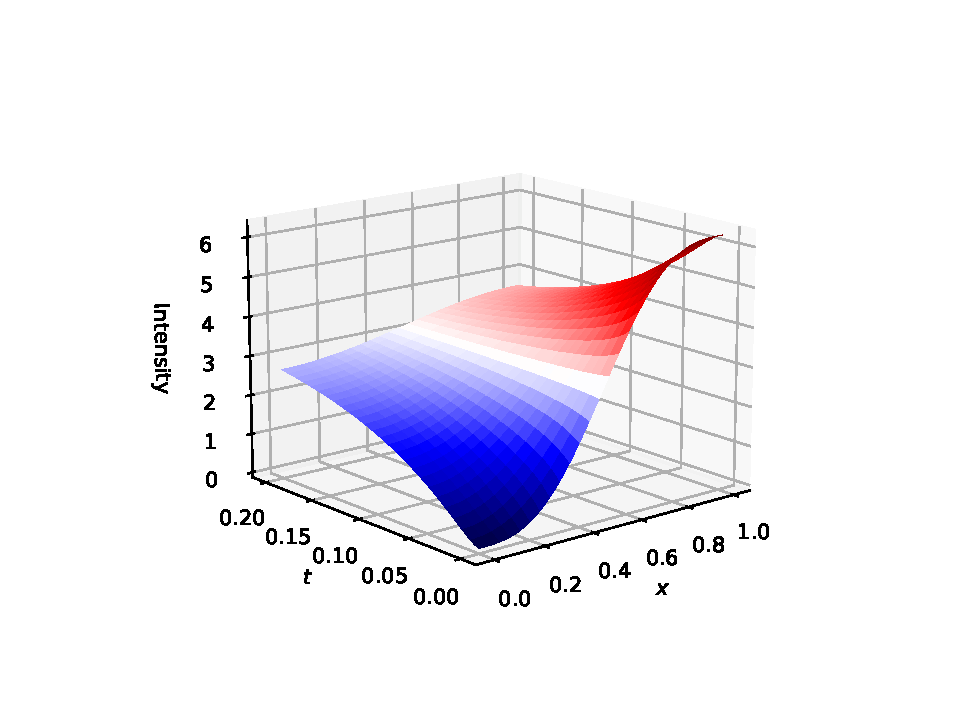
\includegraphics[width = \linewidth]{plots/2a_sol.pdf}
    \caption{Heat equation with two Neumann boundary conditions and initial condition $u(x,0) = 2\pi x - \sin{(2\pi x)}$. The numerical solution is plotted, where second order discretizations of the boundary conditions and CN is used to calculate it.}
    \label{2a_sol}
\end{figure}

\begin{figure}[t]
    \centering
    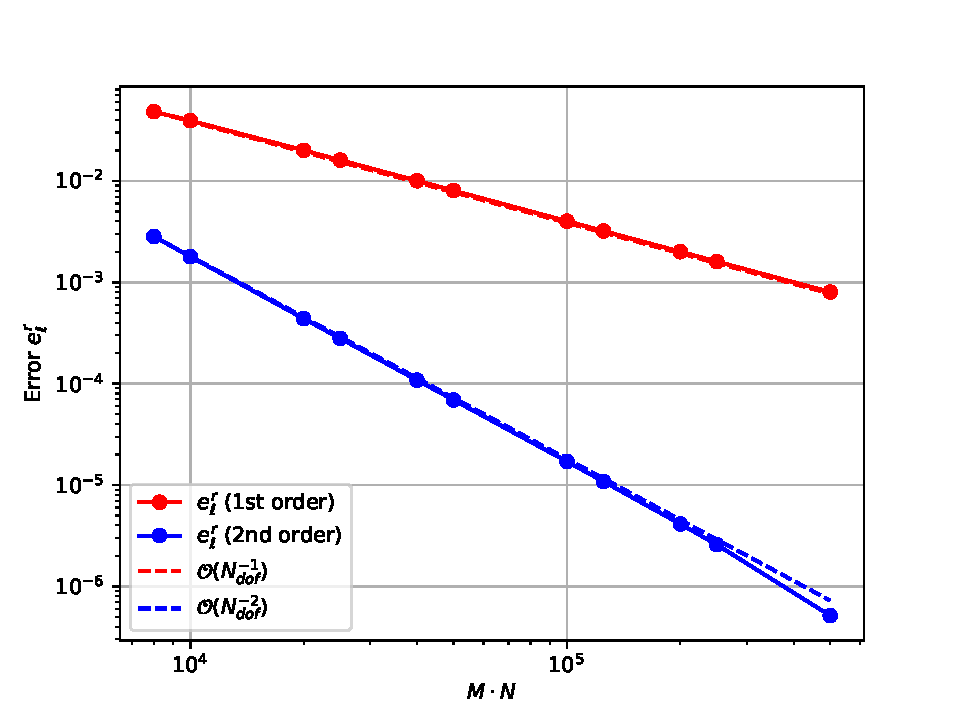
\includegraphics[width = 0.85\linewidth]{plots/2a_comp.pdf}
    \caption{Heat equation with two Neumann boundary conditions and one Dirichlet initial condition. The relative error with $h$-refinement for first and second order discretization of boundary conditions.  \textcolor{red}{Legg gjerne inn $\ell$ og $\mathcal{O}$ i figuren. Jeg har også brukt $\cdot$ på x-aksen ser jeg.}}
    \label{2a_comp}
\end{figure}
\end{comment}


\subsubsection{Convergence Plots}
For this problem, the analytical solution is not available in a closed form. Thus, in order to make convergence plots, a \textit{reference solution}, $\boldsymbol{u}_{M^*}(t)$, must be constructed. It is called a reference solution, since it is a numerical solution with a large number of points $M = M^*$ (small $h = h^*$) in the $x$-direction. Hence, it should be more precise than numerical solutions computed on grids with lower resolutions, which is why it is used as a replacement for the analytical solution when making convergence plots. Throughout this problem, this reference solution has been calculated using $M^* = 1000$ with second order discretizations of the boundary conditions, in combination with CN.

\begin{figure}
\centering
\subfloat[$h$-refinement]{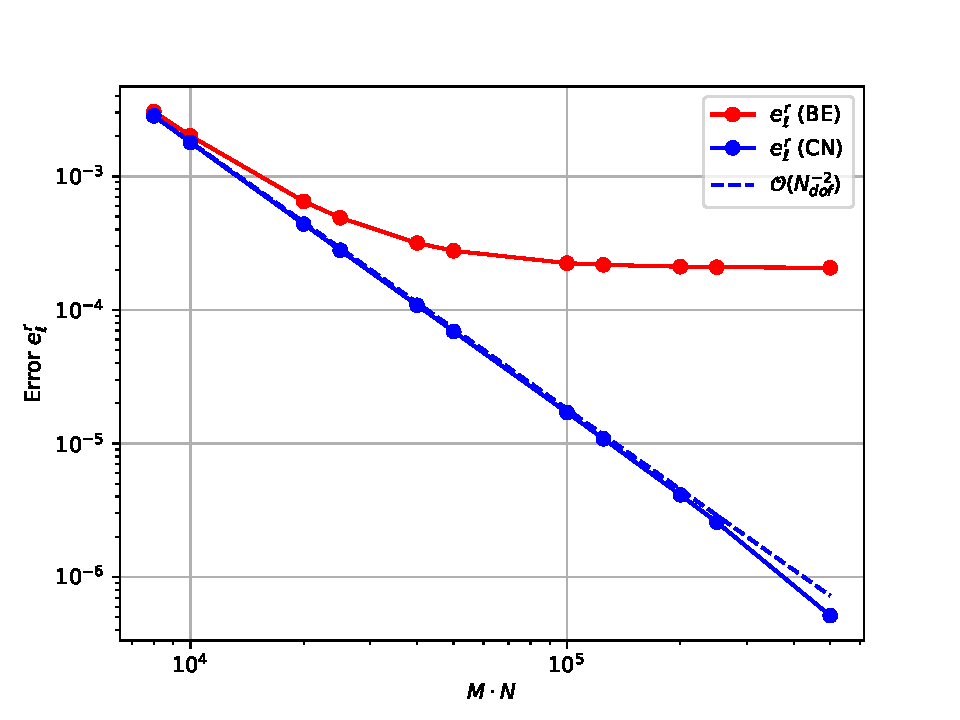
\includegraphics[width=0.85\linewidth]{plots/2a_href.pdf}\label{2a_href}}\hspace{0mm}
\subfloat[$k$-refinement]{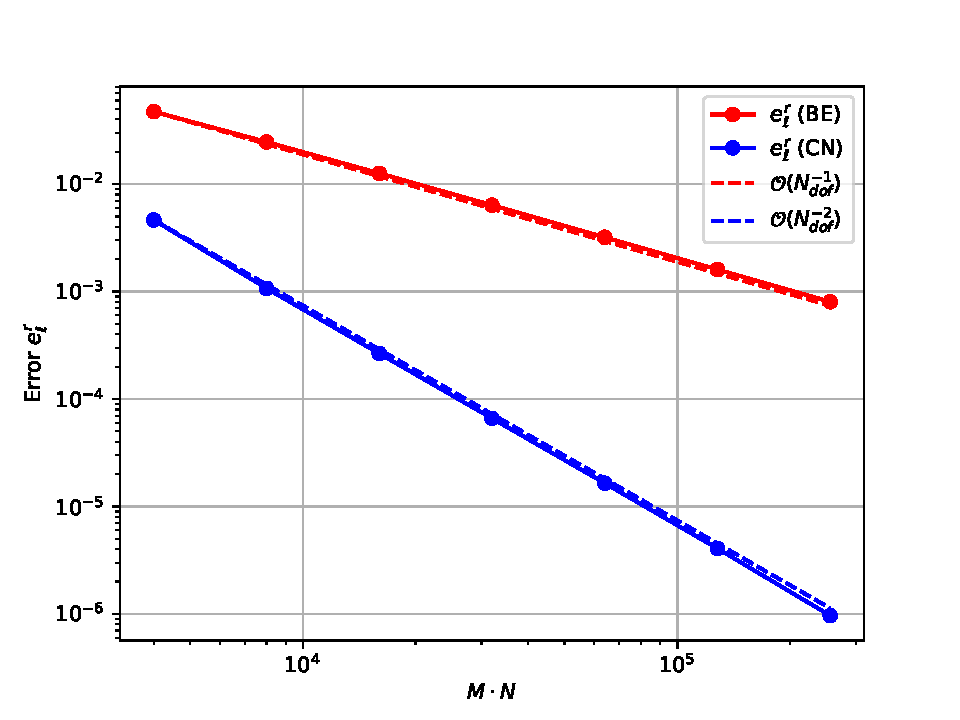
\includegraphics[width=0.85\linewidth]{plots/2a_kref.pdf}\label{2a_kref}}\hspace{0mm}
\caption{Heat equation with two Neumann boundary conditions and initial condition $u(x,0) = 2\pi x - \sin{(2\pi x)}$ on $x \in [0,1]$ and $t \in [0,0.2]$. The relative error obtained with $h$-refinement, with $N=1000$, is plotted in (a). Similarly, the relative error obtained with $k$-refinement, with $M=1000$, is plotted in (b). A second order discretization of the boundary conditions is used when calculating the numerical solution with both BE and CN. The $x$-axis shows the number of degrees of freedom in the linear system.}
\label{fig:2a_hrefAndKref}
\end{figure}

First, how the order of the boundary condition discretization impacts the convergence order with $h$-refinement, is investigated. CN is used, in order to minimize the error in time. The relative error $e_{\ell}^r$, as defined in equation \eqref{discreteRelativeError}, is calculated when increasing the resolution in the $x$-direction. Remember that the analytical solution is replaced by the reference solution in the relative error. The result is depicted in figure \ref{2a_comp}. It is apparent that a first order discretization of the boundary conditions results in first order convergence, even though the finite difference scheme used on the remaining grid points is of second order. Hence, use of the first order discretization of the boundary conditions will be avoided in the following. 

Next, $h$-refinement is considered with both BE and CN. The relative errors are computed and plotted in figure \ref{2a_href}. It is apparent that CN yields second order convergence, while the relative error for BE stagnates at a certain level. This is because BE is less accurate in time; the truncation error for BE is of order one, while for CN it is of order two, as seen in equation \eqref{orders}. In other words, the error in time is dominating the error in BN, which yields no decrease in the relative error when further increasing the spatial resolution. The point of stagnation of the decrease in the relative error for BE could be postponed to a larger number of degrees of freedom and a smaller error by, e.g., increasing the number of time steps $N$.

Furthermore, $k$-refinement, i.e. refinement along the $t$-axis, is considered. The relative errors are computed and plotted in figure \ref{2a_kref}. Note that CN yields second order convergence, while BE yields first order convergence. This is as expected from equation \eqref{orders}, because, in theory, $M$ is set to a large number ($M = 1000$ in the figure), such that the error in $x$ can be neglected, i.e. $\mathcal{O}(k^2 + h^2) = \mathcal{O}(k^2)$ and $\mathcal{O}(k + h^2) = \mathcal{O}(k)$ for CN and BE respectively. 

Finally, $h \propto k$-refinement is considered, This means that the step lengths are proportional, while they are increased at the same rate. The relative errors are calculated and the resulting convergence plot is depicted in figure \ref{rref_2a}. Note that CN yields convergence of first order, while BE yields convergence of order $\frac{1}{2}$. This is in accordance with the expected theoretical convergence orders, which are

\begin{equation*}
    \tau_{CN} = \mathcal{O}(k^2 + h^2) \overset{k \propto h} = \mathcal{O}(kh) = \mathcal{O}\left(\frac{1}{MN}\right) = \mathcal{O}(N_{\mathrm{dof}}^{-1}),
\end{equation*}
and 

\begin{equation*}
    \tau_{BE} = \mathcal{O}(k + h^2) \overset{k \propto h} = \mathcal{O}(h) = \mathcal{O}\left(\frac{1}{M}\right) = \mathcal{O}(N_{\mathrm{dof}}^{-1/2}).
\end{equation*}

\begin{figure}[t]
    \centering
    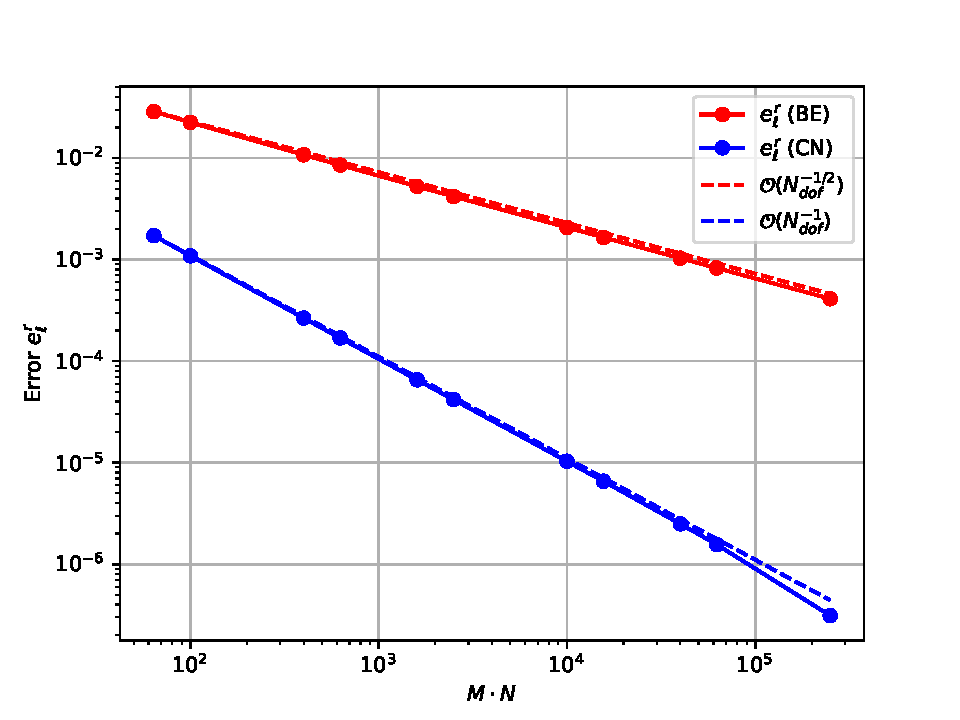
\includegraphics[width = 0.85\linewidth]{plots/rref_BEvsCN1.pdf}
    \caption{Heat equation with two Neumann boundary conditions and initial condition $u(x,0) = 2\pi x - \sin{(2\pi x)}$ on $x \in [0,1]$ and $t \in [0,0.2]$. The relative error obtained with $h \propto k$-refinement, is plotted. CN and a second order discretization of the boundary conditions is used when calculating the numerical solution. The $x$-axis shows the number of degrees of freedom in the linear system.}
    \label{rref_2a}
\end{figure}


\newpage
\subsubsection{b)}
In this subsection, the heat equation 
\begin{equation}
\begin{split}
    &u_t = u_{xx} \hspace{2mm} \text{in} \hspace{2mm} \Omega(x,t): x \in [0,1], t \in [0,T], \\ &u(0,t)=u(1,t)=0,
\label{2b}
\end{split}
\end{equation}
will be solved. $T = 0.2$ is used in the following. By Fourier analysis, a general solution is on the form \cite{Kreyszig}
\begin{equation*}
    u(x,t) = \sum_{n=1}^{\infty} D_n e^{-\pi^2 n^2 t} \sin{(n \pi x)}.
\end{equation*}
Given an initial value $u(x,0)=f(x)$, the coefficients $D_n$ can be determined using the sine orthogonality

\begin{equation*}
    D_n = 2 \int_{0}^{1} f(x) \sin{(n \pi x)} \mathrm{d}x.
\end{equation*}
Now, for simplicity, the initial value $f(x)=3\sin{(2 \pi x)}$ is chosen, which yields a simple manufactured solution on the form 

\begin{equation}
\label{2b-analytical-solution}
    u(x,t) = 3 e^{-4 \pi^2 t} \sin{(2 \pi x)}, 
\end{equation}
since $D_n = 0, \hspace{1mm} \forall n \in \{1\} \cup [3, \infty)$, and $D_2 = \frac12$.
The numerical and manufactured solution is plotted in figure \ref{fig: 2b_sol}.
\begin{figure}[t]
    \centering
    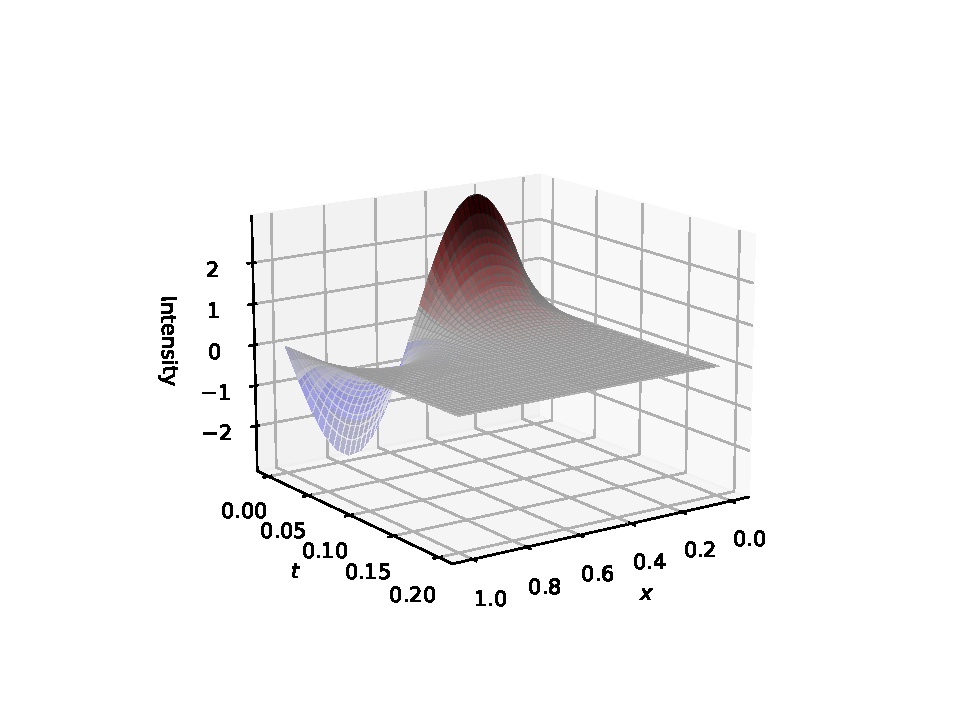
\includegraphics[width = 0.9\linewidth]{plots/2b_sol.pdf}
    \caption{Heat equation on $x \in [0,1]$ and $t \in [0,0.2]$ with homogeneous Dirichlet boundary conditions and initial condition $f(x)=3\sin{(2\pi x)}$. The numerical solution is calculated with CN with $M=N=20$ and plotted with a \textit{seismic} color map. The manufactured solution $u(x,t) = 3 e^{-4 \pi^2 t} \sin{(2 \pi x)}$ is plotted in grey.}
    \label{fig: 2b_sol}
\end{figure}

\subsubsection{Convergence Plots}
In the implementation of the numerical methods, both BE and CN are used to yield a method of second order in space, and first and second order in time, respectively (see equation \eqref{orders}). This means that the schemes \eqref{CN} and \eqref{BE}, with the matrix $Q$ on the form 

\begin{equation*}
Q = \begin{pmatrix}
    -2 & 1 & & & \\
    1 & -2 & 1 & & \\
    & \ddots & \ddots & \ddots &\\
     & & 1 & -2 & 1 \\
     &  & & 1 & -2
    \end{pmatrix}, 
\end{equation*}
are employed. 

\textcolor{red}{Les over dette senere ;)}
We shall consider four types of refinement, namely $h$-, $k$-, $(h=ck)$- and $r$-refinement. Their convergence rates is found by calculating the relative errors in both the $\ell_2$ and $L_2$ norm. The definitions for $e_{\ell}^r$ and $e_{L_2}^r$ can be found in section \ref{errors.section}. The errors are calculated with respect to the analytical solution \eqref{2b-analytical-solution} at the end time for our interval, $T=0.2$, every time the grid is refined. For each type of refinement do we calculate the convergence for both the BE and CN method.

First, $h$-refinement is performed. The convergence plot is depicted in figure \ref{2b_href}. As in problem 2 \mathbf{a)}, the error reaches a minimum when BE is used, due to the error in time. Nevertheless, it can be seen that the convergence is of order 2 when increasing $N$, which is expected from \eqref{orders}, because, in theory, $N$ is set to a large number ($N = 1000$ in the figure) such that the error in $t$ can be neglected, i.e. $\mathcal{O}(k^2 + h^2) = \mathcal{O}(h^2) = \mathcal{O}(N_{\mathrm{dof}}^{-2})$ and $\mathcal{O}(k + h^2) = \mathcal{O}(h^2) = \mathcal{O}(N_{\mathrm{dof}}^{-2})$ for CN and BE respectively. 

Next, $k$-refinement is performed. The convergence plot is depicted in figure \ref{2b_kref}. The convergence plot is in compliance with the truncation orders mentioned in equation \eqref{orders}. The theory predicts these convergence rates because, in theory, $M$ is set to a large number ($M = 1000$ in the figure), such that the error in $x$ can be neglected, i.e. $\mathcal{O}(k^2 + h^2) = \mathcal{O}(k^2) = \mathcal{O}(N_{\mathrm{dof}}^{-2})$ and $\mathcal{O}(k + h^2) = \mathcal{O}(k) = \mathcal{O}(N_{\mathrm{dof}}^{-1})$ for CN and BE respectively.

\begin{figure}
\centering
\subfloat[$h$-refinement]{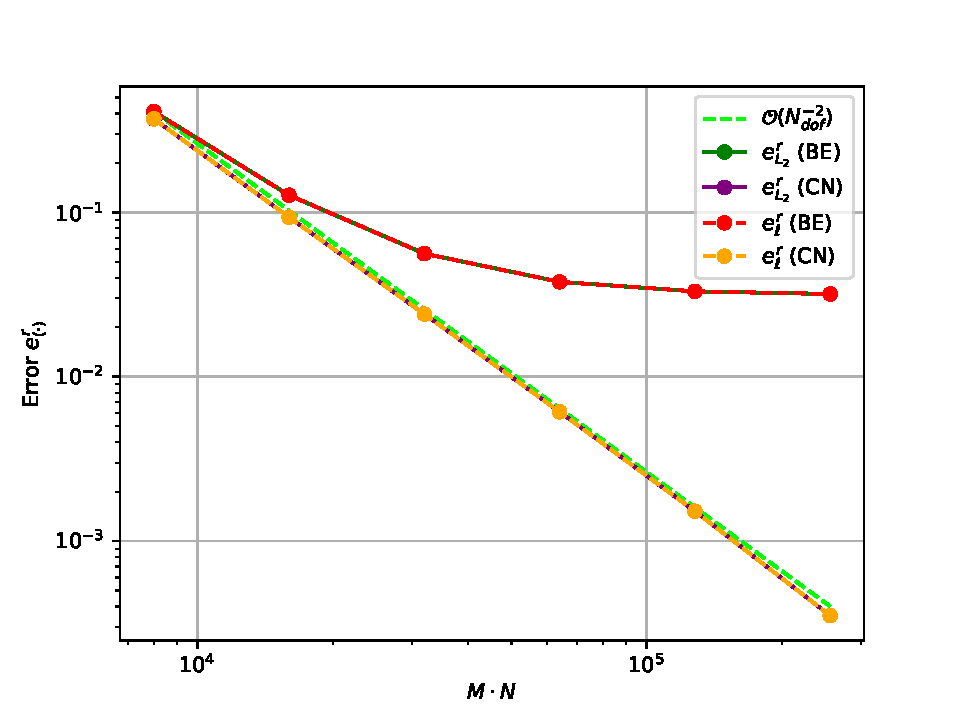
\includegraphics[width=0.85\linewidth]{plots/2b_href.pdf}\label{2b_href}}\hspace{0mm}
\subfloat[$k$-refinement]{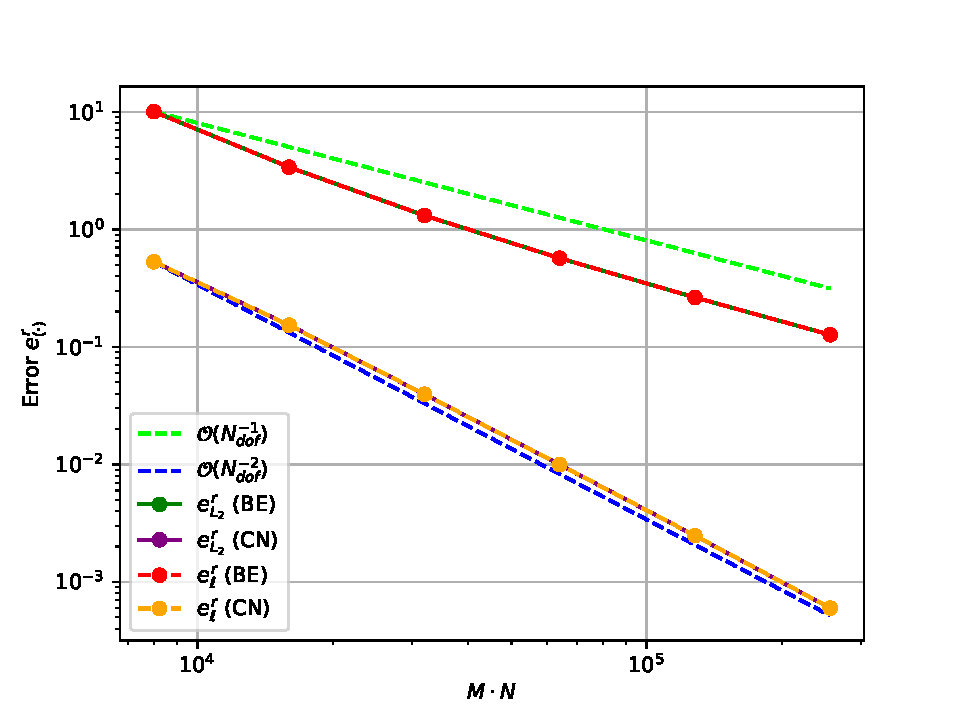
\includegraphics[width=0.85\linewidth]{plots/2b_kref.pdf}\label{2b_kref}}\hspace{0mm}
\caption{ Heat equation with homogeneous Dirichlet boundary conditions, with a manufactured solution $u(x,t) = 3 e^{-4 \pi^2 t} \sin{(2 \pi x)}$, on $x \in [0, 1]$ and $t \in [0, 0.2]$. The relative errors $e_\ell^r$ and $e_{L_2}^r$, obtained with $h$-refinement, are plotted in (a) with $N = 1000$. The relative errors, obtained with $k$-refinement, are plotted in (b) with $M = 1000$. Both BE and CN have been used as integrators. The $x$-axis shows $M \cdot N$, i.e. the number of degrees of freedom of the linear system.}
\end{figure}

Next, mesh refinement where $h = ck$, where $c := 1$, is performed.  From equation \eqref{orders}, it is expected that CN should yield a convergence of order $\mathcal{O}(k^2 + h^2) \overset{k \propto h} = \mathcal{O}(kh) = \mathcal{O}(N_{\mathrm{dof}}^{-1})$. On the other hand, BE is expected to yield convergence of order $\mathcal{O}(k + h^2) \overset{k \propto h} = \mathcal{O}(N_{\mathrm{dof}}^{-\frac{1}{2}} + N_{\mathrm{dof}}^{-1}) = \mathcal{O}(N_{\mathrm{dof}}^{-\frac{1}{2}} )$. The relative errors for both BE and CN are displayed in the convergence plot in figure \ref{2b_r1ref}, which shows that the expectations are met.

\begin{figure}
\centering
\subfloat[$(h = k)$-refinement]{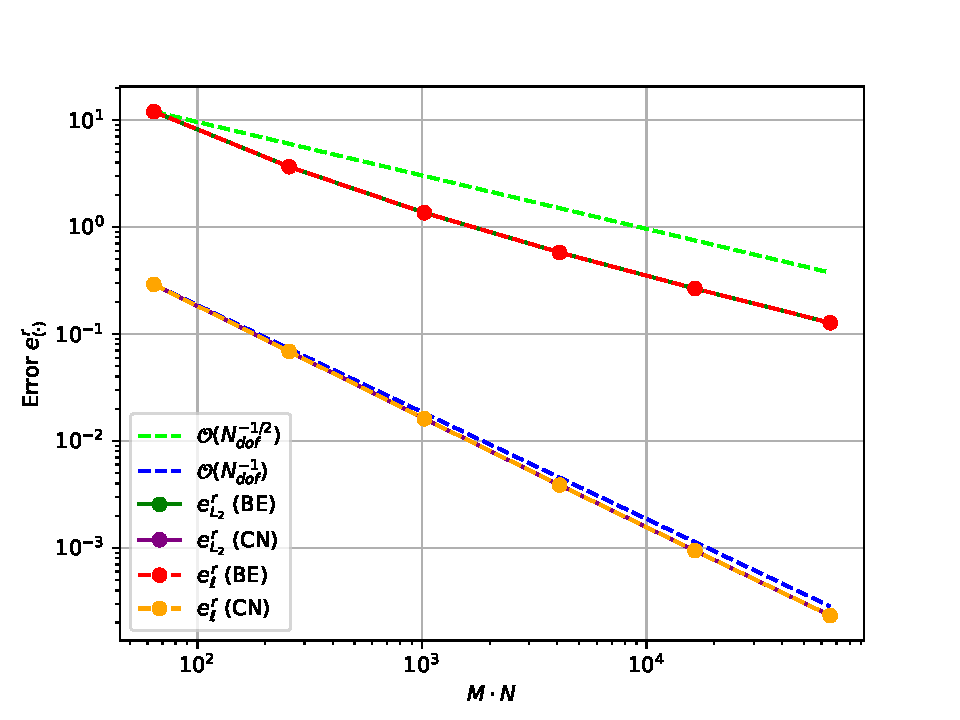
\includegraphics[width=0.85\linewidth]{plots/2b_r1ref.pdf}\label{2b_r1ref}}\hspace{0mm}\subfloat[Mesh refinement with $r = k/h^2$ constant]{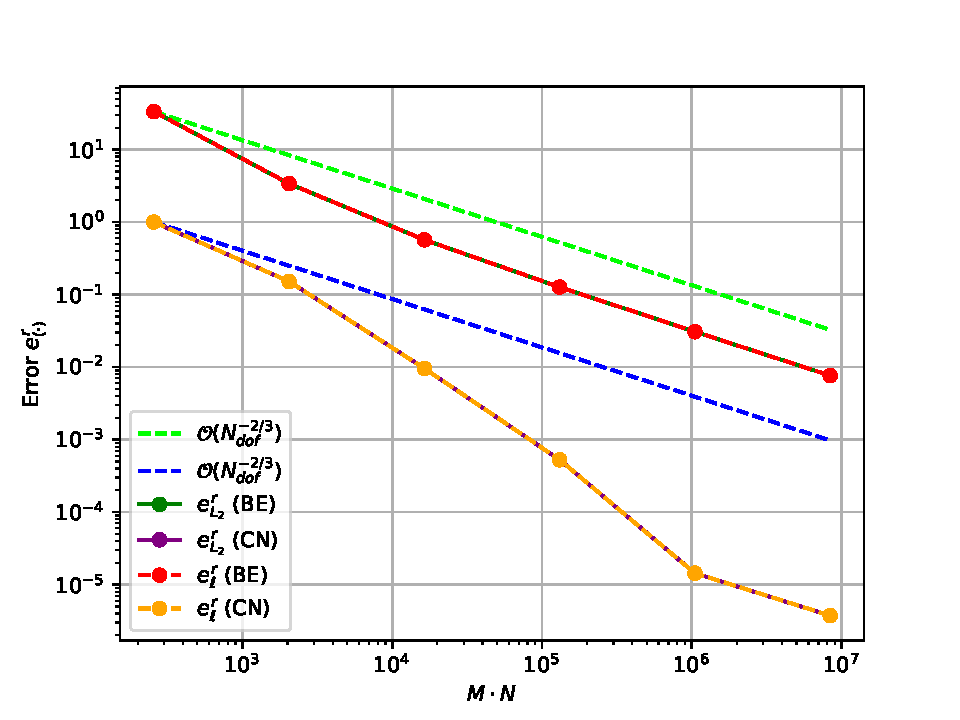
\includegraphics[width=0.85\linewidth]{plots/2b_r2ref.pdf}\label{2b_r2ref}}\hspace{0mm}
\caption{Heat equation with homogeneous Dirichlet boundary conditions, with a manufactured solution $u(x,t) = 3 e^{-4 \pi^2 t} \sin{(2 \pi x)}$, on $x \in [0, 1]$ and $t \in [0, 0.2]$. The relative errors $e_\ell^r$ and $e_{L_2}^r$, obtained with $(h = k)$-refinement, are plotted in (a). The relative errors, obtained with $r = k/h^2$-refinement, are plotted in (b). Both BE and CN have been used as integrators. The $x$-axis shows $M \cdot N$, i.e. the number of degrees of freedom of the linear system.}
\end{figure}

Finally, mesh refinement where $r = \frac{k}{h^2}$ is held constant, is performed. Notice that this implies that $k \propto h^2$ and hence $hk \propto h^3$. Thus, from equation \eqref{orders}, CN is expected to yield convergence of order

\begin{equation*}
    \begin{split}
        \mathcal{O}(k^2 + h^2) &\overset{k^2 \propto h^4}= \mathcal{O}(h^4 + h^2) \\ 
        = \mathcal{O}(h^2) &\overset{hk \propto h^3}= \mathcal{O}((hk)^{\frac{2}{3}}) = \mathcal{O}(N_{\mathrm{dof}}^{-\frac{2}{3}}).
    \end{split}
\end{equation*}
BE is expected to yield the same order of convergence

\begin{equation*}
    \begin{split}
        \mathcal{O}(k + h^2) &= \mathcal{O}(h^2) = \mathcal{O}((hk)^{\frac{2}{3}}) = \mathcal{O}(N_{\mathrm{dof}}^{-\frac{2}{3}}).
    \end{split}
\end{equation*}
The relative errors for both BE and CN are displayed in the convergence plot in figure \ref{2b_r2ref}, which shows that the expectations are partly met.

\newpage
\subsubsection{c)}
The inviscid Burgers' equation

\begin{equation}
    u_t = -uu_x, \, u(0,t) = u(1,t) = 0, \, u(x,0) = \exp{(-400(x-1/2)^2)},
\label{2c.burger}
\end{equation}
will be considered on $x \in [0,1], \, t > 0$. This is a special case of the parabolic Burgers' equation

\begin{equation*}
    u_t = \epsilon u_{xx} - uu_x, \, \epsilon \rightarrow 0.
\end{equation*}
The $x$-axis is discretized such that

\begin{equation*}
    x_0 = 0, \, x_1 = \frac{1}{M+1}, \, \dots, \, x_M = \frac{M}{M+1}, \, x_{M+1} = 1.
\end{equation*}
Let $v_m(t) \approx u(x_m,t)$ for $0 \leq m \leq M+1$ be the numerical solution along the line $(x_m,t)$. Using a central difference approximation for the first spatial derivative, which, from section \ref{section_2.2}, is known to be a second order approximation, leads to 

\begin{equation}
    \dot{v}_m =  - v_m\frac{1}{2h}(v_{m+1}-v_{m-1}), \quad 1 \le m \le M,
\label{burger_disc}
\end{equation}

\noindent All these differential equations can be written in vector format with $\boldsymbol{v}=[v_1,v_2,\dots,v_M]^T$. Combining the boundary conditions $v_0=v_{M+1}=0$  with \eqref{burger_disc} gives 

\begin{equation}
    \dot{\boldsymbol{v}} =: \boldsymbol{F}(\boldsymbol{v}) = \frac{1}{2h} \begin{pmatrix}
    -v_1v_2 \\
    \vdots \\
    -v_m(v_{m+1} - v_{m-1}) \\
    \vdots \\
    v_{M}v_{M-1}
    \end{pmatrix}
\label{2c.ODE}
\end{equation}

\noindent The system \eqref{2c.ODE} is solved in time with the ODE-solving method RK4. For a detailed description of the RK4 method see chapter 4. This yields a breaking time in the interval $t^* \in [0.057,0.060]$, which agrees with the theoretical value of $t^* = -1/ \min\{u'(x,0)\} \approx 0.0583$ found in \cite{Burgers}. Figure \ref{2c.fig} shows a visualization of the breaking point of the numerical solution. 

\begin{figure}[t]
    \centering
    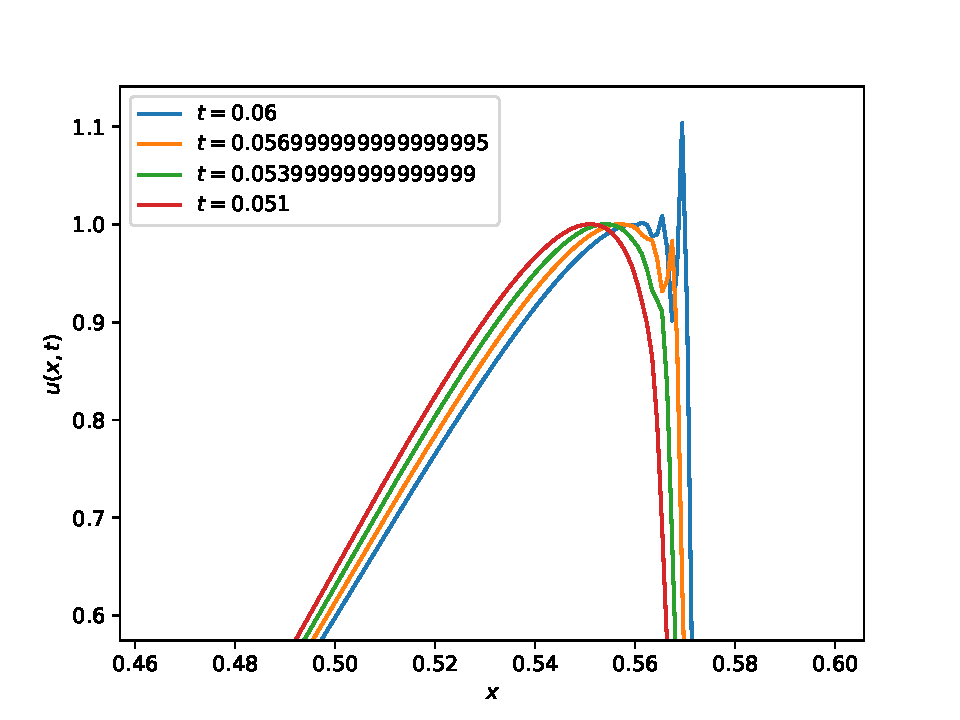
\includegraphics[width = 0.85\linewidth]{plots/2c.pdf}
    \caption{Inviscid Burger's equation on $x \in [0,1], \, t > 0$, with homogeneous Dirichlet boundary conditions and one initial condition. The numerical solution is plotted along the $x$-axis for different values of $t$. The plot illustrates the "breaking" behavior of the solution. }
    \label{2c.fig}
\end{figure}
\newpage
\ 
\newpage
\newpage
\ 
\newpage
